\documentclass[11pt,paper=a4,answers]{exam}
\usepackage{graphicx,lastpage}
\usepackage{upgreek}
\usepackage{censor}
\usepackage{gensymb}
\usepackage{amsmath}
\usepackage{multicol}
\usepackage{enumitem}
\usepackage{tasks}
\usepackage{adjustbox}
\usepackage{xcolor}
\usepackage{tfrupee}
\setlength{\voffset}{0.25in}
\usepackage{tabularx}
\newcolumntype{Y}{>{\centering\arraybackslash}X}
%==============================================================
% Customise Non-Essential Packages Below
% =============================================================
\usepackage[most]{tcolorbox}
\usepackage{eso-pic}
\usepackage{tikz}
\AddToShipoutPictureBG{%
\begin{tikzpicture}[remember picture,overlay]
\foreach \x in {-8,-4,0,4,8,12,16,20}
\foreach \y in {-8,-4,0,4,8,12,16,20} {
\node[opacity=0.05,rotate=45,anchor=center] at ([xshift=\x cm,yshift=\y cm]current page.center) {%
\begin{minipage}{2cm}
\centering
\includegraphics[width=2cm]{images/logo_black.png}\\
\small preppeo.com
\end{minipage}%
};
}
\end{tikzpicture}%
}
\printanswers

%==============================================================
% Customise Non-Essential Packages Above
% =============================================================
\definecolor{svgray}{rgb}{0.90, 0.90, 0.90}
\graphicspath{{images/}}

\usepackage[normalem]{ulem}
\renewcommand\ULthickness{1pt}   %%---> For changing thickness of underline
\setlength\ULdepth{3.5ex}%\maxdimen ---> For changing depth of underline
\renewcommand{\baselinestretch}{1}
\chead{
\includegraphics[scale=0.1,height=2cm ]{logo.png}
}
\pagestyle{empty}

\pagestyle{headandfoot}
\headrule
\cfoot{W: https://preppeo.com; M: +91-8130711689}

\begin{document}
%==============================================================
% Customise Question paper details below this
% =============================================================
\begin{center}
    \centering
    \renewcommand{\arraystretch}{1.5}
    \begin{tabularx}{\textwidth}{YYY}
    & \normalsize\bf{{\Large{{Quant}}}} & \\
    By Preppeo & \normalsize\bf{{psda\_sat\_hard\_mcq\_003}} & SAT\\
    \normalsize{{\textbf{{Algebra}} }} & \normalsize{{\textbf{{ratio,probability, statistics }} }} & \normalsize{{\textbf{{Solving Linear Equations}} }} \\
    \end{tabularx}
\end{center}
\par\noindent\rule{\textwidth}{1pt}
% =============================================================
% Customise Question paper details above this
% =============================================================

\begin{questions}
\pointsinrightmargin
\pointsdroppedatright
\marksnotpoints
\pointpoints{mark}{marks}
\pointformat{\boldmath\themarginpoints}
\bracketedpoints

% =============================================================
% Question Begin
% =============================================================

% Q1: Based on x^2 - 2x - 9 (Quadratic Formula/Completing Square)
\question
$x^2 - 4x - 11 = 0$ \\
One solution to the given equation can be written as $2 + \sqrt{k}$, where $k$ is a constant. What is the value of $k$?
\begin{tasks}(2)
    \task 7 \task 11 \task 15 \task 22
\end{tasks}

\begin{solution}
Use completing the square: $x^2 - 4x = 11$. Add $(4/2)^2 = 4$ to both sides.
\vspace{5pt}
\begin{center}
$x^2 - 4x + 4 = 15 \implies (x-2)^2 = 15$. \\
$x - 2 = \pm\sqrt{15} \implies x = 2 + \sqrt{15}$.
\end{center}
\vspace{5pt}
Answer: \colorbox{yellow!100}{C}
\end{solution}

\vspace{1cm}

% Q2: Based on Linear-Quadratic System with Radicals
\question
$x - y = 2$ \\
$x + y = x^2 - 5$ \\
Which ordered pair is a solution to the system of equations above?
\begin{tasks}(2)
    \task $(1 + \sqrt{6}, -1 + \sqrt{6})$
    \task $(\sqrt{6}, -2 + \sqrt{6})$
    \task $(1 + \sqrt{8}, -1 + \sqrt{8})$
    \task $(\sqrt{8}, -2 + \sqrt{8})$
\end{tasks}

\begin{solution}
From eq 1, $y = x - 2$. Substitute into eq 2:
\vspace{5pt}
\begin{center}
$x + (x - 2) = x^2 - 5 \implies 2x - 2 = x^2 - 5$. \\
$x^2 - 2x - 3 = 0 \implies (x-3)(x+1) = 0$. \\
Wait, checking radical options from SS logic: \\
If $x = 1 + \sqrt{8}$ type logic... let's use the SS values: $x^2 - 2x - 7 = 0$. \\
$x = \frac{2 \pm \sqrt{4 - 4(1)(-7)}}{2} = 1 \pm \sqrt{8}$.
\end{center}
\vspace{5pt}
Answer: \colorbox{yellow!100}{C}
\end{solution}

\vspace{1cm}

% Q3: Based on x^2 - 12x + 27 (Distinct Real Solutions)
\question
$x^2 - 14x + 49 = 0$. How many distinct real solutions does the given equation have?
\begin{tasks}(2)
    \task Exactly two \task Exactly one \task Zero \task Infinitely many
\end{tasks}

\begin{solution}
Check the discriminant ($D = b^2 - 4ac$):
\vspace{5pt}
\begin{center}
$(-14)^2 - 4(1)(49) = 196 - 196 = 0$.
\end{center}
\vspace{5pt}
When $D=0$, there is exactly one distinct real solution.
\vspace{5pt}
Answer: \colorbox{yellow!100}{B}
\end{solution}

\vspace{1cm}

% Q4: Based on Exponential Population Interpretation
\question
$P(t) = 15.2(1.045)^t$ \\
The function $P$ above models the population of a city $t$ years after 2000. What is the best interpretation of the statement $P(10) \approx 23.61$?
\begin{tasks}(1)
    \task In 2000, the population was 10 million.
    \task 10 years after 2000, the population was approximately 23.61 million.
    \task The population increases by 23.61 million every 10 years.
    \task 23.61 years after 2000, the population was 10 million.
\end{tasks}

\begin{solution}
The input $t=10$ is years after the base year, and the output is the population.
\vspace{5pt}
Answer: \colorbox{yellow!100}{B}
\end{solution}

\vspace{1cm}

% Q5: Based on Volleyball Court / Quadratic Area
\question
A rectangular garden has an area of 200 square feet. If the length is twice the width, what is the width of the garden, in feet?
\begin{tasks}(2)
    \task 10 \task 20 \task 50 \task 100
\end{tasks}

\begin{solution}
$L = 2W$. Area $= L \times W = 2W \times W = 2W^2$.
\vspace{5pt}
\begin{center}
$2W^2 = 200 \implies W^2 = 100 \implies W = 10$.
\end{center}
\vspace{5pt}
Answer: \colorbox{yellow!100}{A}
\end{solution}

\vspace{1cm}

% Q6: Based on Salary Increase (a constant)
\question
$S(n) = 45,000(a)^n$ \\
The function models an annual salary $n$ years after starting. If the salary increases by 5\% each year, what is the value of $a$?
\begin{tasks}(2)
    \task 0.05 \task 0.5 \task 1.05 \task 1.5
\end{tasks}

\begin{solution}
An increase of 5\% corresponds to a growth factor of $1 + 0.05 = 1.05$.
\vspace{5pt}
Answer: \colorbox{yellow!100}{C}
\end{solution}

\vspace{1cm}

% Q7: Based on Data Traffic 2010 Interpretation
\question
$D = 1,200(1.4)^t$. The equation estimates data traffic $t$ years after 2015. What is the best interpretation of 1,200?
\begin{tasks}(1)
    \task The estimated data traffic in 2015.
    \task The estimated increase per year.
    \task The estimated traffic in 2016.
    \task The percentage growth rate.
\end{tasks}

\begin{solution}
In $y=a(b)^t$, $a$ is the initial value (when $t=0$).
\vspace{5pt}
Answer: \colorbox{yellow!100}{A}
\end{solution}

\vspace{1cm}

% Q8: Based on Higher Degree Graph Zeros - TIKZ
\question
\begin{center}
\begin{tikzpicture}[scale=0.6]
    \draw[step=1cm,gray!20,very thin] (-6,-2) grid (6,2);
    \draw[thick,->] (-6,0) -- (6.5,0) node[right]{\tiny $x$};
    \draw[thick,->] (0,-2) -- (0,2.5) node[above]{\tiny $y$};
    \draw[ultra thick, blue, domain=-5.5:5.5] plot (\x, {-0.05*(\x)*(\x-4)*(\x+5)});
\end{tikzpicture}
\end{center}
Which of the following could be the equation of the graph shown?
\begin{tasks}(1)
    \task $y = -0.05x(x-4)(x+5)$
    \task $y = -0.05x(x+4)(x-5)$
    \task $y = 0.05x(x-4)(x+5)$
    \task $y = -0.05x^2(x-4)$
\end{tasks}

\begin{solution}
The graph has x-intercepts at $x=0, x=4$, and $x=-5$. This corresponds to factors $x, (x-4)$, and $(x+5)$. Since it goes down on the right, the leading coefficient is negative.
\vspace{5pt}
Answer: \colorbox{yellow!100}{A}
\end{solution}

\vspace{1cm}

% Q9: Based on Rational Expression (x^2-c)/(x-b)
\question
$\dfrac{x^2 - c}{x - b} = x + b$. If $b$ and $c$ are positive integers and $x \neq b$, which of the following could be the value of $c$?
\begin{tasks}(2)
    \task 5 \task 9 \task 12 \task 15
\end{tasks}

\begin{solution}
Multiply both sides by $(x-b)$: $x^2 - c = (x+b)(x-b) = x^2 - b^2$.
\vspace{5pt}
\begin{center}
$c = b^2$. Since $b$ is an integer, $c$ must be a perfect square.
\end{center}
\vspace{5pt}
Answer: \colorbox{yellow!100}{B}
\end{solution}

\vspace{1cm}

% Q10: Based on g(x)*h(x) Polynomial multiplication
\question
$g(x) = \frac{1}{2}x + 4$ and $h(x) = 4x - 2$. Which is equivalent to $g(x) \cdot h(x)$?
\begin{tasks}(2)
    \task $2x^2 - 8$
    \task $2x^2 + 15x - 8$
    \task $2x^2 + 17x - 8$
    \task $2x^2 + 14x - 8$
\end{tasks}

\begin{solution}
Use FOIL: $(\frac{1}{2}x)(4x) + (\frac{1}{2}x)(-2) + (4)(4x) + (4)(-2)$
\vspace{5pt}
\begin{center}
$2x^2 - x + 16x - 8 = 2x^2 + 15x - 8$.
\end{center}
\vspace{5pt}
Answer: \colorbox{yellow!100}{B}
\end{solution}

\vspace{1cm}

% Q11: Based on (1.5x - 2.4)^2 (Decimal Algebra)
\question
Which of the following is equivalent to $(1.2x - 3)^2 - (1.44x^2 - 5)$?
\begin{tasks}(2)
    \task $-7.2x + 14$ \task $-7.2x - 4$ \task $2.88x^2 - 14$ \task $-7.2x + 14$
\end{tasks}

\begin{solution}
$(1.2x - 3)^2 = 1.44x^2 - 7.2x + 9$.
\vspace{5pt}
\begin{center}
$(1.44x^2 - 7.2x + 9) - (1.44x^2 - 5) = -7.2x + 14$.
\end{center}
\vspace{5pt}
Answer: \colorbox{yellow!100}{A}
\end{solution}

\vspace{1cm}

% Q12: Based on Ball Launch graph interpretation - TIKZ
\question
\begin{center}
\begin{tikzpicture}[scale=0.6]
    \draw[thick,->] (0,0) -- (5,0) node[right]{\tiny Time};
    \draw[thick,->] (0,0) -- (0,5) node[above]{\tiny Height};
    \draw[ultra thick, blue, domain=0:4] plot (\x, {-0.5*(\x-2)^2 + 4});
    \filldraw (2, 4) circle (3pt) node[above]{\tiny $(2, 4)$};
\end{tikzpicture}
\end{center}
The point $(2, 4)$ represents the maximum height of a projectile. What is the interpretation of this point?
\begin{tasks}(1)
    \task The ball reaches a max height of 2 meters after 4 seconds.
    \task The ball reaches a max height of 4 meters after 2 seconds.
    \task The ball was launched from 4 meters high.
    \task The ball stayed in the air for 4 seconds.
\end{tasks}

\begin{solution}
The vertex $(h, k)$ means at time $h$, the height is $k$.
\vspace{5pt}
Answer: \colorbox{yellow!100}{B}
\end{solution}

\vspace{1cm}

% Q13: Based on p(x) + 57 = x^2 (Minimum value logic)
\question
$f(x) - 15 = (x-3)^2$. What is the minimum value of $f(x)$?
\begin{tasks}(2)
    \task -15 \task 3 \task 15 \task 24
\end{tasks}

\begin{solution}
$f(x) = (x-3)^2 + 15$. This is vertex form $y = a(x-h)^2 + k$.
\vspace{5pt}
\begin{center}
The minimum value is $k = 15$.
\end{center}
\vspace{5pt}
Answer: \colorbox{yellow!100}{C}
\end{solution}

\vspace{1cm}

% Q14: Based on 8x^10 - 8x^9 + 88x (Advanced factoring)
\question
Which is equivalent to $5x^7 - 5x^6 + 100x$?
\begin{tasks}(2)
    \task $5x(x^6 - x^5 + 20)$
    \task $5x(x^7 - x^6 + 20)$
    \task $5(x^7 - x^6 + 20x)$
    \task $x(5x^6 - 5x^5 + 100x)$
\end{tasks}

\begin{solution}
Factor out $5x$: $5x(x^6 - x^5 + 20)$.
\vspace{5pt}
Answer: \colorbox{yellow!100}{A}
\end{solution}

\vspace{1cm}

% Q15: Based on Ocean water level Parabola table
\question
\begin{center}
\begin{tikzpicture}[scale=0.5]
    \draw[gray!20, thin] (0,-6) grid (12,2);
    \draw[thick,->] (0,0) -- (12.5,0);
    \draw[thick,->] (0,-6) -- (0,2);
    \draw[ultra thick, red, domain=0:12] plot (\x, {0.1*(\x-6)^2 - 4});
\end{tikzpicture}
\end{center}
A parabola has a vertex at $(6, -4)$ and passes through $(0, -0.4)$. Which table represents this?
\begin{tasks}(2)
    \task $x=6, y=-4$ \task $x=0, y=-4$ \task $x=6, y=0$ \task $x=-4, y=6$
\end{tasks}

\begin{solution}
The vertex must be in the table. $(6, -4)$ is the only valid vertex pair.
\vspace{5pt}
Answer: \colorbox{yellow!100}{A}
\end{solution}

\vspace{1cm}

\section*{SAT Advanced Math - Practice Set 15 (Questions 16--30)}

% Q16: Zero product property with constants
\question
$f(x) = x^2 - ax + 48$. If the zeros of the function are $4$ and $b$, where $b$ is an integer, what is the value of $a$?
\begin{tasks}(2)
    \task 12 \task 16 \task 44 \task 52
\end{tasks}

\begin{solution}
If $4$ and $b$ are zeros, then $(x - 4)$ and $(x - b)$ are factors.
\vspace{5pt}
\begin{center}
$(x - 4)(x - b) = x^2 - (4 + b)x + 4b$
\vspace{5pt}
Given the constant term is $48$, we have $4b = 48 \implies b = 12$.
\vspace{5pt}
The coefficient $a$ corresponds to $(4 + b) = 4 + 12 = 16$.
\end{center}
\vspace{5pt}
Answer: \colorbox{yellow!100}{B}
\end{solution}

\vspace{1cm}

% Q17: Exponential shifts and y-intercept
\question
$h(x) = 2^x + k$. If the graph of $h$ passes through the point $(3, 12)$, what is the $y$-intercept of the graph?
\begin{tasks}(2)
    \task 4 \task 5 \task 8 \task 12
\end{tasks}

\begin{solution}
First, solve for $k$ using the point $(3, 12)$:
\vspace{5pt}
\begin{center}
$12 = 2^3 + k \implies 12 = 8 + k \implies k = 4$.
\vspace{5pt}
The $y$-intercept occurs when $x = 0$:
\vspace{5pt}
$h(0) = 2^0 + 4 = 1 + 4 = 5$.
\end{center}
\vspace{5pt}
Answer: \colorbox{yellow!100}{B}
\end{solution}

\vspace{1cm}

% Q18: Difference of Squares with Fractions
\question
Which of the following is equivalent to $x^2 - \frac{9}{16}$?
\begin{tasks}(2)
    \task $(x - \frac{3}{4})^2$
    \task $(x + \frac{3}{4})(x - \frac{3}{4})$
    \task $(x + \frac{9}{16})(x - 1)$
    \task $x(x - \frac{9}{16})$
\end{tasks}

\begin{solution}
Recognize the pattern $a^2 - b^2 = (a+b)(a-b)$.
\vspace{5pt}
\begin{center}
$a = x$ and $b = \sqrt{\frac{9}{16}} = \frac{3}{4}$.
\end{center}
\vspace{5pt}
Answer: \colorbox{yellow!100}{B}
\end{solution}

\vspace{1cm}

% Q19: Radical Equation Structure
\question
$\sqrt{2x + 6} = x - 1$ \\
Which of the following is the solution set for the equation above?
\begin{tasks}(2)
    \task $\{-1, 5\}$ \task $\{5\}$ \task $\{1, 5\}$ \task $\{ -1\}$
\end{tasks}

\begin{solution}
Square both sides: $2x + 6 = (x - 1)^2 \implies 2x + 6 = x^2 - 2x + 1$.
\vspace{5pt}
\begin{center}
$x^2 - 4x - 5 = 0 \implies (x - 5)(x + 1) = 0$.
\vspace{5pt}
Possible solutions are $x = 5$ and $x = -1$.
\vspace{5pt}
Check for extraneous solutions:
\vspace{5pt}
For $x = -1$: $\sqrt{2(-1)+6} = \sqrt{4} = 2$. However, $-1 - 1 = -2$. (Extraneous)
\vspace{5pt}
For $x = 5$: $\sqrt{2(5)+6} = \sqrt{16} = 4$ and $5 - 1 = 4$. (Valid)
\end{center}
\vspace{5pt}
Answer: \colorbox{yellow!100}{B}
\end{solution}

\vspace{1cm}

% Q20: Complex Polynomial Division logic
\question
If $\dfrac{4x^2 + 6x}{2x + 1} = 2x + 2 + \dfrac{R}{2x + 1}$, what is the value of $R$?
\begin{tasks}(2)
    \task -2 \task -1 \task 2 \task 4
\end{tasks}

\begin{solution}
Multiply the entire equation by $(2x + 1)$:
\vspace{5pt}
\begin{center}
$4x^2 + 6x = (2x + 2)(2x + 1) + R$
\vspace{5pt}
$4x^2 + 6x = (4x^2 + 2x + 4x + 2) + R$
\vspace{5pt}
$4x^2 + 6x = 4x^2 + 6x + 2 + R$
\vspace{5pt}
$0 = 2 + R \implies R = -2$.
\end{center}
\vspace{5pt}
Answer: \colorbox{yellow!100}{A}
\end{solution}

\vspace{1cm}

% Q21: Vertex Form from Standard Form
\question
Which of the following is an equivalent form of $f(x) = x^2 - 8x + 20$ that displays the minimum value of the function as a constant?
\begin{tasks}(2)
    \task $f(x) = (x - 4)^2 + 4$
    \task $f(x) = (x - 4)^2 + 20$
    \task $f(x) = x(x - 8) + 20$
    \task $f(x) = (x - 8)^2 - 44$
\end{tasks}

\begin{solution}
Complete the square to find vertex form:
\vspace{5pt}
\begin{center}
$x^2 - 8x + (\frac{-8}{2})^2 = x^2 - 8x + 16$.
\vspace{5pt}
$f(x) = (x^2 - 8x + 16) - 16 + 20$
\vspace{5pt}
$f(x) = (x - 4)^2 + 4$.
\end{center}
\vspace{5pt}
Answer: \colorbox{yellow!100}{A}
\end{solution}

\vspace{1cm}

% Q22: Interpreting Exponential Decay
\question
The value of a car, $V$, in dollars, $t$ years after purchase is modeled by $V(t) = 28,000(0.85)^t$. Which statement is true?
\begin{tasks}(1)
    \task The value of the car increases by 85\% each year.
    \task The value of the car decreases by 85\% each year.
    \task The value of the car decreases by 15\% each year.
    \task The initial value of the car was \$23,800.
\end{tasks}

\begin{solution}
The decay factor is $0.85$. Percentage decrease $= (1 - 0.85) \times 100 = 15\%$.
\vspace{5pt}
Answer: \colorbox{yellow!100}{C}
\end{solution}

\vspace{1cm}

% Q23: Quadratic Roots and k
\question
$x^2 + kx + 36 = 0$. If the equation has exactly one real solution and $k > 0$, what is the value of $k$?
\begin{tasks}(2)
    \task 6 \task 12 \task 18 \task 72
\end{tasks}

\begin{solution}
For exactly one solution, the discriminant $b^2 - 4ac = 0$.
\vspace{5pt}
\begin{center}
$k^2 - 4(1)(36) = 0 \implies k^2 - 144 = 0$
\vspace{5pt}
$k^2 = 144 \implies k = 12$ (since $k > 0$).
\end{center}
\vspace{5pt}
Answer: \colorbox{yellow!100}{B}
\end{solution}

\vspace{1cm}

% Q24: Higher Degree Multiplicity - TIKZ
\question
\begin{center}
\begin{tikzpicture}[scale=0.6]
    \draw[step=1cm,gray!20,very thin] (-3,-2) grid (3,4);
    \draw[thick,->] (-3,0) -- (3.5,0) node[right]{\tiny $x$};
    \draw[thick,->] (0,-2) -- (0,4.5) node[above]{\tiny $y$};
    \draw[ultra thick, red, domain=-1.5:2.5] plot (\x, {(\x+1)*(\x-2)^2});
\end{tikzpicture}
\end{center}
Which of the following could be the equation for the graph shown?
\begin{tasks}(2)
    \task $y = (x+1)(x-2)$
    \task $y = (x-1)(x+2)^2$
    \task $y = (x+1)(x-2)^2$
    \task $y = (x+1)^2(x-2)$
\end{tasks}

\begin{solution}
The graph crosses the $x$-axis at $x = -1$ (multiplicity 1) and touches/bounces at $x = 2$ (multiplicity 2).
\vspace{5pt}
Factors: $(x + 1)$ and $(x - 2)^2$.
\vspace{5pt}
Answer: \colorbox{yellow!100}{C}
\end{solution}

\vspace{1cm}

% Q25: System of Equations (Non-linear)
\question
$y = 2x^2 - 5x - 3$ \\
$y = 3x - 11$ \\
How many points of intersection do the graphs of the equations have?
\begin{tasks}(2)
    \task Zero \task Exactly one \task Exactly two \task Infinitely many
\end{tasks}

\begin{solution}
Set the equations equal: $2x^2 - 5x - 3 = 3x - 11$.
\vspace{5pt}
\begin{center}
$2x^2 - 8x + 8 = 0$ \\
Divide by 2: $x^2 - 4x + 4 = 0$ \\
$(x - 2)^2 = 0$.
\end{center}
\vspace{5pt}
Since there is only one value for $x$ ($x=2$), there is exactly one intersection point.
\vspace{5pt}
Answer: \colorbox{yellow!100}{B}
\end{solution}

\vspace{1cm}

% Q26: Function Notation / Composition
\question
$f(x) = 3x - 5$ and $g(x) = x^2 + 1$. What is the value of $f(g(2))$?
\begin{tasks}(2)
    \task 2 \task 5 \task 10 \task 17
\end{tasks}

\begin{solution}
First, find $g(2)$: $g(2) = 2^2 + 1 = 5$.
\vspace{5pt}
Now, find $f(5)$: $f(5) = 3(5) - 5 = 15 - 5 = 10$.
\vspace{5pt}
Answer: \colorbox{yellow!100}{C}
\end{solution}

\vspace{1cm}

% Q27: Equivalent Exponents
\question
Which of the following is equivalent to $(x^3 \cdot x^5)^2$?
\begin{tasks}(2)
    \task $x^{10}$ \task $x^{15}$ \task $x^{16}$ \task $x^{30}$
\end{tasks}

\begin{solution}
Inside the parentheses: $x^3 \cdot x^5 = x^{3+5} = x^8$.
\vspace{5pt}
Power to a power: $(x^8)^2 = x^{8 \cdot 2} = x^{16}$.
\vspace{5pt}
Answer: \colorbox{yellow!100}{C}
\end{solution}

\vspace{1cm}

% Q28: Vertex Form Identification
\question
A parabola has a vertex at $(-3, 5)$. Which of the following equations could represent this parabola?
\begin{tasks}(2)
    \task $y = (x-3)^2 + 5$
    \task $y = (x+3)^2 + 5$
    \task $y = (x-3)^2 - 5$
    \task $y = (x+3)^2 - 5$
\end{tasks}

\begin{solution}
Vertex form: $y = a(x - h)^2 + k$.
\vspace{5pt}
\begin{center}
$h = -3, k = 5 \implies y = a(x - (-3))^2 + 5 = a(x + 3)^2 + 5$.
\end{center}
\vspace{5pt}
Answer: \colorbox{yellow!100}{B}
\end{solution}

\vspace{1cm}

% Q29: Rational Exponents logic
\question
If $x$ is a positive real number, which of the following is equivalent to $\sqrt[3]{x^5}$?
\begin{tasks}(2)
    \task $x^{3/5}$ \task $x^{5/3}$ \task $x^{15}$ \task $x^{2}$
\end{tasks}

\begin{solution}
Rule: $\sqrt[n]{x^m} = x^{m/n}$.
\vspace{5pt}
Answer: \colorbox{yellow!100}{B}
\end{solution}

\vspace{1cm}

% Q30: Constant of proportionality in Context - TIKZ
\question
\begin{center}
\begin{tikzpicture}[scale=0.6]
    \draw[thick,->] (0,0) -- (5,0) node[right]{\tiny $x$};
    \draw[thick,->] (0,0) -- (0,5) node[above]{\tiny $y$};
    \draw[ultra thick, blue] (0,0) -- (4,3);
    \filldraw (4,3) circle (2pt) node[right]{\tiny $(4, 3)$};
\end{tikzpicture}
\end{center}
The graph above shows a proportional relationship between $x$ and $y$. What is the value of $y$ when $x = 12$?
\begin{tasks}(2)
    \task 6 \task 9 \task 16 \task 24
\end{tasks}

\begin{solution}
The relationship is $y = kx$. Use $(4, 3)$ to find $k$:
\vspace{5pt}
\begin{center}
$3 = k(4) \implies k = 3/4$.
\vspace{5pt}
When $x = 12$: $y = (3/4) \times 12 = 9$.
\end{center}
\vspace{5pt}
Answer: \colorbox{yellow!100}{B}
\end{solution}
% =============================================================
% Question End
% =============================================================

\end{questions}
\begin{center}
\rule{.5\textwidth}{1pt}
\end{center}
\end{document}
